\documentclass[journal,10pt,twocolumn]{IEEEtran}

\usepackage[utf8]{inputenc}
\usepackage{kvmap}
\usepackage{graphics} 

\usepackage{setspace}
\usepackage{gensymb}

\singlespacing



\usepackage{amsthm}

\usepackage{mathrsfs}
\usepackage{txfonts}
\usepackage{stfloats}
\usepackage{bm}
\usepackage{cite}
\usepackage{cases}
\usepackage{subfig}

\usepackage{longtable}
\usepackage{multirow}

\usepackage{enumitem}
\usepackage{mathtools}
\usepackage{steinmetz}
\usepackage{tikz}
\usepackage{circuitikz}
\usepackage{verbatim}
\usepackage{tfrupee}
\usepackage[colorlinks=true,  linkcolor=blue, urlcolor=blue]{hyperref}
\usepackage{graphicx}
\usepackage{tkz-euclide}
\usepackage{float}

\usetikzlibrary{calc,math}
\usepackage{listings}
    \usepackage{color}                                            %%
    \usepackage{array}                                            %%
    \usepackage{longtable}                                        %%
    \usepackage{calc}                                             %%
    \usepackage{multirow}                                         %%
    \usepackage{hhline}                                           %%
    \usepackage{ifthen}                                           %%
    \usepackage{lscape}     
\usepackage{multicol}
\usepackage{chngcntr}


\usepackage{graphicx}
\usepackage[margin=0.5in]{geometry}
\usepackage{amssymb}
\usepackage{array}
\usepackage{booktabs}
\usepackage{mathtools}
\usepackage{dirtree}
\usepackage{xcolor}
\usepackage{float}
\usepackage[justification=centering,font={rm,md,scriptsize}]{caption}
\usepackage{enumitem}
\usepackage{listings}
\usepackage{mathtools}
\usepackage{fancyvrb}
%\usepackage{hyperref}


%Add chapter functionality in IEEEtran class
\newcounter{Chapcounter}
\newcommand\showmycounter{\addtocounter{Chapcounter}{1}\themycounter}
\newcommand{\chapter}[1] 
{ {\centering          
  \addtocounter{Chapcounter}{1} \large \textbf{Chapter \theChapcounter ~#1}}  
  \addcontentsline{toc}{section}{Chapter ~\theChapcounter~~ #1}    
  \setcounter{section}{0}
}
%%%%



\numberwithin{equation}{subsection}
\numberwithin{figure}{subsection}

\counterwithin{enumi}{subsection}
\counterwithin{equation}{subsection}
\counterwithin{figure}{subsection}


\renewcommand\thesection{\theChapcounter.\arabic{section}}
\renewcommand\thesectiondis{\theChapcounter.\arabic{section}}
\newcommand\figref{Fig.~\ref}

\setenumerate{label=\thesection.\arabic*}

\lstset{
  basicstyle=\ttfamily,
  columns=fullflexible,
  frame=single,
  breaklines=true,
  postbreak=\mbox{\textcolor{red}{$\hookrightarrow$}\space},
}

\providecommand{\mbf}{\mathbf}
\providecommand{\pr}[1]{\ensuremath{\Pr\left(#1\right)}}
\providecommand{\qfunc}[1]{\ensuremath{Q\left(#1\right)}}
\providecommand{\sbrak}[1]{\ensuremath{{}\left[#1\right]}}
\providecommand{\lsbrak}[1]{\ensuremath{{}\left[#1\right.}}
\providecommand{\rsbrak}[1]{\ensuremath{{}\left.#1\right]}}
\providecommand{\brak}[1]{\ensuremath{\left(#1\right)}}
\providecommand{\lbrak}[1]{\ensuremath{\left(#1\right.}}
\providecommand{\rbrak}[1]{\ensuremath{\left.#1\right)}}
\providecommand{\cbrak}[1]{\ensuremath{\left\{#1\right\}}}
\providecommand{\lcbrak}[1]{\ensuremath{\left\{#1\right.}}
\providecommand{\rcbrak}[1]{\ensuremath{\left.#1\right\}}}
\newcommand{\sgn}{\mathop{\mathrm{sgn}}}
\providecommand{\abs}[1]{\left\vert#1\right\vert}
\providecommand{\res}[1]{\Res\displaylimits_{#1}} 
\providecommand{\norm}[1]{\left\lVert#1\right\rVert}
\providecommand{\mtx}[1]{\mathbf{#1}}
\providecommand{\mean}[1]{E\left[ #1 \right]}
\providecommand{\fourier}{\overset{\mathcal{F}}{ \rightleftharpoons}}
\providecommand{\ztrans}{\overset{\mathcal{Z}}{ \rightleftharpoons}}
\providecommand{\system}{\overset{\mathcal{H}}{ \longleftrightarrow}}
\newcommand{\solution}{\noindent \textbf{Solution: }}
\newcommand{\cosec}{\,\text{cosec}\,}
\providecommand{\dec}[2]{\ensuremath{\overset{#1}{\underset{#2}{\gtrless}}}}
\newcommand{\myvec}[1]{\ensuremath{\begin{pmatrix}#1\end{pmatrix}}}
\newcommand{\mydet}[1]{\ensuremath{\begin{vmatrix}#1\end{vmatrix}}}
\providecommand{\gauss}[2]{\mathcal{N}\ensuremath{\left(#1,#2\right)}}
\newcommand*{\permcomb}[4][0mu]{{{}^{#3}\mkern#1#2_{#4}}}
\newcommand*{\perm}[1][-3mu]{\permcomb[#1]{P}}
\newcommand*{\comb}[1][-1mu]{\permcomb[#1]{C}}

\let\vec\mathbf

\def\putbox#1#2#3{\makebox[0in][l]{\makebox[#1][l]{}\raisebox{\baselineskip}[0in][0in]{\raisebox{#2}[0in][0in]{#3}}}}
     \def\rightbox#1{\makebox[0in][r]{#1}}
     \def\centbox#1{\makebox[0in]{#1}}
     \def\topbox#1{\raisebox{-\baselineskip}[0in][0in]{#1}}
     \def\midbox#1{\raisebox{-0.5\baselineskip}[0in][0in]{#1}}


\DeclareMathOperator*{\Res}{Res}

\renewcommand\thesection{\arabic{section}}
\renewcommand\thesubsection{\thesection.\arabic{subsection}}
\renewcommand\thesubsubsection{\thesubsection.\arabic{subsubsection}}

\renewcommand\thesectiondis{\arabic{section}}
\renewcommand\thesubsectiondis{\thesectiondis.\arabic{subsection}}
\renewcommand\thesubsubsectiondis{\thesubsectiondis.\arabic{subsubsection}}


\hyphenation{op-tical net-works semi-conduc-tor}
\def\inputGnumericTable{}                                 %%

\lstset{
%language=C,
frame=single, 
breaklines=true,
columns=fullflexible
}
\begin{document}


\title{Digital Communcation Assignment}

\author{Surabhi Seetha}
\date{January 2022}

\maketitle

\tableofcontents

\bigskip

% CHAPTER 1

\section{Two Dice}
\subsection{\textbf{Sum of Independent Random Variables}}
Two dice, one blue and one grey, are thrown at the same time.   The event defined by the sum of the two numbers appearing on the top of the dice can have 11 possible outcomes 2, 3, 4, 5, 6, 7, 8, 9, 10, 11 and 12.  A student argues that each of these outcomes has a probability $\frac{1}{11}$.  Do you agree with this argument?  Justify your answer.
\begin{enumerate}[label=\thesubsection.\arabic*.,ref=\thesubsection.\arabic{figure}]
%\numberwithin{equation}{enumi}
%\numberwithin{figure}{enumi}
\item {\em The Uniform distribution} Let $X_i \in \cbrak{1,2,3,4,5,6}, i = 1,2,$ be the random variables representing the outcome for each die.  Assuming the dice to be fair, the probability mass function (pmf) is expressed as 
\begin{align}
\label{eq:dice_pmf_xi}
p_{X_i}(n) = \pr{X_i = n} =
\begin{cases}
\frac{1}{6} & 1 \le n \le 6
\\
0 & otherwise
\end{cases}
\end{align}
The desired outcome is
\begin{align}
\label{eq:dice_xdef}
X &= X_1 + X_2,
\\
\implies X &\in \cbrak{1,2,\dots,12}
\end{align}
The objective is to show that
\begin{align}
p_X(n) \ne \frac{1}{11}
\label{eq:dice_wrong}
\end{align}
\item {\em Convolution: }
From \eqref{eq:dice_xdef},
\begin{align}
p_X(n) &= \pr{X_1 + X_2 = n} = \pr{X_1  = n -X_2}
\\
&= \sum_{k}^{}\pr{X_1  = n -k | X_2 = k}p_{X_2}(k)
\label{eq:dice_x_sum}
\end{align}
after unconditioning.  $\because X_1$ and $X_2$ are independent,
\begin{multline}
\pr{X_1  = n -k | X_2 = k} 
\\
= \pr{X_1  = n -k} = p_{X_1}(n-k)
\label{eq:dice_x1_indep}
\end{multline}
From \eqref{eq:dice_x_sum} and \eqref{eq:dice_x1_indep},
\begin{align}
p_X(n) = \sum_{k}^{}p_{X_1}(n-k)p_{X_2}(k) = p_{X_1}(n)*p_{X_2}(n)
\label{eq:dice_x_conv}
\end{align}
where $*$ denotes the convolution operation. 
%\cite{proakis_dsp}.  
Substituting from \eqref{eq:dice_pmf_xi}
in \eqref{eq:dice_x_conv},
\begin{align}
p_X(n) = \frac{1}{6}\sum_{k=1}^{6}p_{X_1}(n-k)= \frac{1}{6}\sum_{k=n-6}^{n-1}p_{X_1}(k)
\label{eq:dice_x_conv_x1}
\end{align}
\begin{align}
\because p_{X_1}(k) &= 0, \quad k \le 1, k \ge 6.
\end{align}
From \eqref{eq:dice_x_conv_x1},
%
\begin{align}
p_X(n) &= 
\begin{cases}
0 & n < 1
\\
\frac{1}{6}\sum_{k=1}^{n-1}p_{X_1}(k) &  1 \le n-1 \le  6
\\
\frac{1}{6}\sum_{k=n-6}^{6}p_{X_1}(k) & 1 < n-6 \le 6
\\
0 & n > 12
\end{cases}
\label{eq:dice_x_conv_cond}
\end{align}
Substituting from \eqref{eq:dice_pmf_xi} in \eqref{eq:dice_x_conv_cond},
\begin{align}
p_X(n) &= 
\begin{cases}
0 & n < 1
\\
\frac{n-1}{36} &  2 \le n \le  7
\\
\frac{13-n}{36} & 7 < n \le 12
\\
0 & n > 12
\end{cases}
\label{eq:dice_x_conv_final}
\end{align}
satisfying \eqref{eq:dice_wrong}.

\item {\em The $Z$-transform: }
The $Z$-transform of $p_X(n)$ is defined as 
%\cite{proakis_dsp}
\begin{align}
P_X(z) = \sum_{n = -\infty}^{\infty}p_X(n)z^{-n}, \quad z \in \mathbb{C}
\label{eq:dice_xz}
\end{align}
%
From \eqref{eq:dice_pmf_xi} and \eqref{eq:dice_xz}, 
\begin{align}
P_{X_1}(z) =P_{X_2}(z) &= \frac{1}{6}\sum_{n = 1}^{6}z^{-n}
\\
&=\frac{z^{-1}\brak{1-z^{-6}}}{6\brak{1-z^{-1}}},  \abs{z} >1
\label{eq:dice_xiz}
\end{align}
upon summing up the geometric progression.  
\begin{align}
\because p_X(n) &= p_{X_1}(n)*p_{X_2}(n),
\\
P_X(z) &= P_{X_1}(z)P_{X_2}(z)
\label{eq:dice_xzprod_def}
\end{align}
The above property follows from Fourier analysis and is fundamental to signal processing. 
%\cite{proakis_dsp}. 
From \eqref{eq:dice_xiz} and \eqref{eq:dice_xzprod_def},
\begin{align}
P_X(z) &= \cbrak{\frac{z^{-1}\brak{1-z^{-6}}}{6\brak{1-z^{-1}}}}^2
\\
&= \frac{1}{36}\frac{z^{-2}\brak{1-2z^{-6}+z^{-12}}}{\brak{1-z^{-1}}^2}
\label{eq:dice_xzprod}
\end{align}
Using the fact that 
%\cite{proakis_dsp}
\begin{align}
p_X(n-k) &\system{Z}P_X(z)z^{-k},
\\
nu(n)&\system{Z} \frac{z^{-1}}{\brak{1-z^{-1}}^2}
\end{align}
after some algebra, it can be shown that
%{\tiny
\begin{multline}
\frac{1}{36}\lsbrak{\brak{n-1}u(n-1) - 2 \brak{n-7}u(n-7)}
\\
\rsbrak{ +\brak{n-13}u(n-13)}
\\
\system{Z}
\frac{1}{36}\frac{z^{-2}\brak{1-2z^{-6}+z^{-12}}}{\brak{1-z^{-1}}^2}
\label{eq:dice_xz_closed}
\end{multline}
%}
where 
\begin{align}
u(n) =
\begin{cases}
1 & n \ge 0
\\
0 & n < 0
\end{cases}
\end{align}
From \eqref{eq:dice_xz}, \eqref{eq:dice_xzprod} and \eqref{eq:dice_xz_closed}
\begin{multline}
p_{X}(n) = \frac{1}{36}\lsbrak{\brak{n-1}u(n-1) 
}
\\
\rsbrak{- 2 \brak{n-7}u(n-7)+\brak{n-13}u(n-13)}
\end{multline}
which is the same as \eqref{eq:dice_x_conv_final}.  Note that  \eqref{eq:dice_x_conv_final} can be obtained from \eqref{eq:dice_xz_closed} using contour integration as well.

\item 
The experiment of rolling the dice was simulated using Python for 10000 samples.  These were generated using Python libraries for uniform distribution. The frequencies for each outcome were then used to compute the resulting pmf, which  is plotted in Figure \ref{fig:dice}.  The theoretical pmf obtained in \eqref{eq:dice_x_conv_final} is plotted for comparison.
\begin{figure}[!ht]
\centering
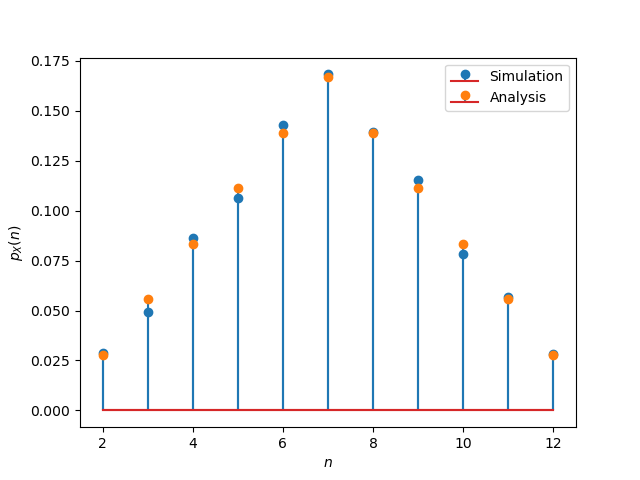
\includegraphics[width=\columnwidth]{/home/vijay/Digital_Communication/Figs/Chapter1/dice.png} 
\caption{Plot of $p_X(n)$ Simulations are close to the Analysis results. }
\label{fig:dice}
\end{figure}

\item The python code is available in\\
\
\fbox{\parbox{85mm}{\href{https://github.com/SurabhiSeetha/Fwciith2022}{/Codes/Chapter1/Dice.py}}}
\end{enumerate}

% CHAPTER 2 

\section{Random Variables}
%\numberwithin{equation}{enumi}
\subsection{\textbf{Uniform Random Numbers}}
Let $U$ be a uniform random variable between 0 and 1.
\begin{enumerate}[label=\thesubsection.\arabic*,ref=\thesubsection.\arabic{figure}]%\theenumi]
\item
Generate $10^6$ samples of $U$ using a C program and save into a file called uni.dat .
\\
\solution Download the following files and execute the  C program.\\
\fbox{\parbox{85mm}{\href{https://github.com/SurabhiSeetha/Fwciith2022}{/Codes/Chapter2/coeffs.h}}}\\
\
\fbox{\parbox{85mm}{\href{https://github.com/SurabhiSeetha/Fwciith2022}{/Codes/Chapter2/uniformgen.c}}}

\item
Load the uni.dat file into python and plot the empirical CDF of $U$ using the samples in uni.dat. The CDF is defined as
\begin{align}
F_{U}(x) = \pr{U \le x}
\end{align}
\solution  The below code gives the plot in \figref{fig:uni_cdf}\\
\
\fbox{\parbox{85mm}{\href{https://github.com/SurabhiSeetha/Fwciith2022}{/Codes/Chapter2/uni$\_$cdf.py}}}

\begin{figure}[!ht]
\centering
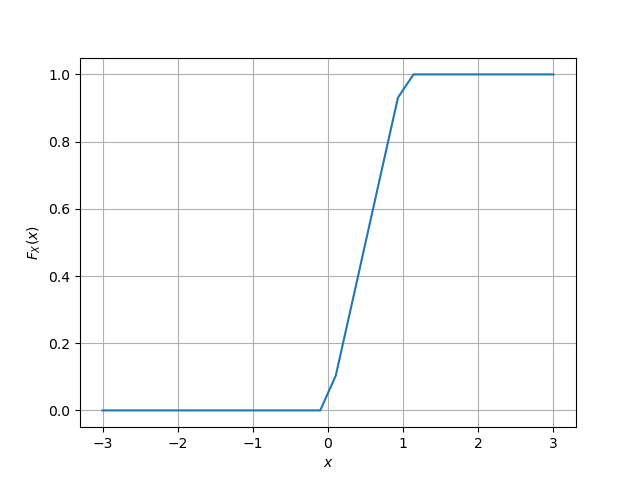
\includegraphics[width=\columnwidth]{/home/vijay/Digital_Communication/Figs/Chapter2/uni_cdf.png}
\caption{The CDF of $U$}
\label{fig:uni_cdf}
\end{figure}

\item
Find a  theoretical expression for $F_{U}(x)$.
\\
\solution
We Know that,
\begin{align} 
F_{U}(x) = \int_{-\infty}^{x} f_{U}(x)\,dx
\label{eq:pdf_to_cdf}
\end{align}
For the uniform random variable $U$, $f_{U}(x)$ is  
\begin{align}
	f_U(x) &= 
	\begin{cases}
	1 &  a \le x \le  b
	\\
	0 & elsewhere
	\\
	\end{cases}
	\label{eq:uni_pdf}
\end{align}
Substituting \eqref{eq:uni_pdf} in \eqref{eq:pdf_to_cdf}, $F_U(x)$ we get
\begin{align}
F_{U}(x) &= 
\begin{cases}
0 & x < a \\
\frac{x-a}{b-a} & a \leq x \leq b \\
1 & x \geq b
\end{cases}
\label{eq:dice_x_conv_final}
\end{align}
were, a=0 and b=1. Hence, \eqref{eq:dice_x_conv_final} can be written as
\begin{align}
	F_U(x) &= 
	\begin{cases}
	0 & x < 0
	\\	
	x & 0 \le x \le  1
	\\
	1 & x > 0
	\\
	\end{cases}
	\label{eq:uniform_cdf}
\end{align}

\item
\label{eq:print_uni}
The mean of $U$ is defined as
%
\begin{equation}
E\sbrak{U} = \frac{1}{N}\sum_{i=1}^{N}U_i
\end{equation}
%
and its variance as
%
\begin{equation}
\text{var}\sbrak{U} = E\sbrak{U- E\sbrak{U}}^2 
\end{equation}
Write a C program to  find the mean and variance of $U$. \\
\solution The following code prints the mean and variance of $U$\\
\
\fbox{\parbox{85mm}{\href{https://github.com/SurabhiSeetha/Fwciith2022}{/Codes/Chapter2/uni$\_$ $mean\_var$.c}}}\\
\
\vspace{0.1cm}

The output of the program is
\begin{lstlisting}
Uniform stats:
Mean: 0.500007
Variance: 0.083301
\end{lstlisting}
\item Verify your result theoretically given that
%
\begin{align}
E\sbrak{U^k} = \int_{-\infty}^{\infty}x^kdF_{U}(x)
\label{eq:expe1}
\end{align}
\solution We Know That, For any given random variable $X$, the mean $\mu_X$ and variance $\sigma_X^2$ are formulated as
\begin{align}
	\label{eq:mean_exp}
	Mean \hspace{0.2cm} \mu_X &= E\sbrak{X} = \int_{-\infty}^{\infty}xdF_{U}(x) \\
	\label{eq:var_exp}
	Variance \hspace{0.2cm} \sigma_X^2 &= E\sbrak{X^2} - \mu_X^2 = \int_{-\infty}^{\infty}x^2dF_{U}(x) - \mu_X^2
\end{align}  
Substituting the CDF of $U$ from \eqref{eq:uniform_cdf} in \eqref{eq:mean_exp} and \eqref{eq:var_exp}, we get
\begin{align}
	\label{eq:mean_uni}
	\mu_U &= \frac{1}{2} \\
	\label{eq:var_uni}
	\sigma_U^2 &= \frac{1}{12}
\end{align}  
which match with the printed values in previous problem.
\end{enumerate}

\subsection{\textbf{Central Limit Theorem}}
%
\begin{enumerate}[label=\thesubsection.\arabic*,ref=\thesubsection.\arabic{figure}]
%
\item
Generate $10^6$ samples of the random variable
%
\begin{equation}
X = \sum_{i=1}^{12}U_i -6
\end{equation}
%
using a C program, where $U_i, i = 1,2,\dots, 12$ are  a set of independent uniform random variables between 0 and 1
and save in a file called gau.dat \\
\solution Download the following files and execute the  C program.\\

\fbox{\parbox{85mm}{\href{https://github.com/SurabhiSeetha/Fwciith2022}{/Codes/Chapter2/coeffs.h}}}\\

\fbox{\parbox{85mm}{\href{https://github.com/SurabhiSeetha/Fwciith2022}{/Codes/Chapter2/gau$\_$gen.c}}}

\
\item
Load gau.dat in python and plot the empirical CDF of $X$ using the samples in gau.dat. What properties does a CDF have?
\\
\solution The CDF of $X$ is plotted in Fig.\ref{fig:gauss_cdf} using the following code.\\

\fbox{\parbox{85mm}{\href{https://github.com/SurabhiSeetha/Fwciith2022}{/Codes/Chapter2/gau$\_$cdf$\_$plot.py}}}\\

\textbf{Properties:}
\begin{itemize}
\item CDF is non-decreasing function\\
\begin{align}
\frac{dF_X(x)}{dx} \ge 0
\end{align}
\item Maximum value of CDF $F(+\infty)=1$.
\item Minimum value of CDF $F(-\infty)=0$.
\end{itemize}
\
\begin{figure}[!ht]
\centering
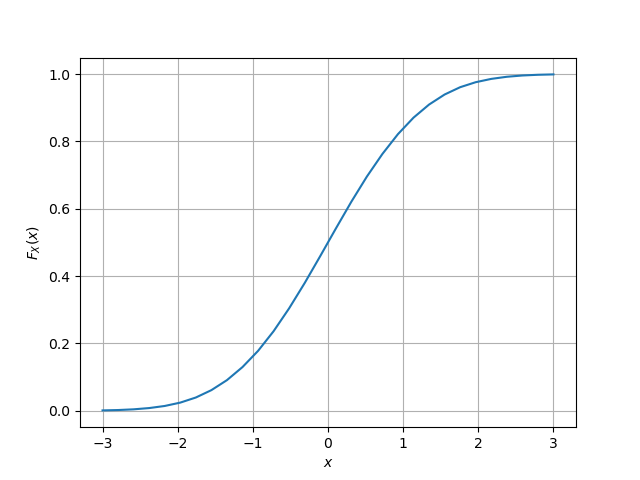
\includegraphics[width=\columnwidth]{/home/vijay/Digital_Communication/Figs/Chapter2/gau_cdf_plot.png}
\caption{The CDF of $X$}
\label{fig:gauss_cdf}
\end{figure}

\item
Load gau.dat in python and plot the empirical PDF of $X$ using the samples in gau.dat. The PDF of $X$ is defined as
\begin{align}
p_{X}(x) = \frac{d}{dx}F_{X}(x)
\label{eq:cdf_to_pdf}
\end{align}
What properties does the PDF have?
\\
\solution The PDF of $X$ is plotted in Fig. \ref{fig:gauss_pdf} using the code below\\

\fbox{\parbox{85mm}{\href{https://github.com/SurabhiSeetha/Fwciith2022}{/Codes/Chapter2/gau$\_$pdf$\_$plot.py}}}\\

\textbf{Properties} : 
\begin{itemize}
\item The PDF is always non-negative
\begin{align}
f_X(x) \ge 0
\end{align}
\item Mean,median and mode are equal.
\item The PDF curve is symmetric about mean.
\item Area under the curve=1.
\begin{align}
	\int_{-\infty}^{\infty} f_X(x) \,dx = 1
\end{align}
\end{itemize}

\begin{figure}[!ht]
\centering
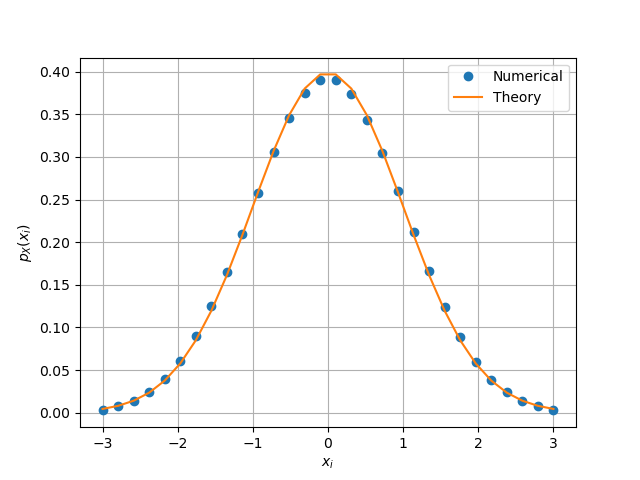
\includegraphics[scale=0.5]{/home/vijay/Digital_Communication/Figs/Chapter2/gau_pdf_plot.png}  
\caption{The PDF of $X$}
\label{fig:gauss_pdf}
\end{figure}

\item Find the mean and variance of $X$ by writing a C program.\\

\solution The following code gives the mean and variance of $X$\\

\fbox{\parbox{85mm}{\href{https://github.com/SurabhiSeetha/Fwciith2022}{/Codes/Chapter2/gau$\_$mean$\_$var.c}}}\\

The outputs are
\begin{lstlisting}
Gaussian stats:
Mean: 0.000294
Variance: 0.999562	
\end{lstlisting}

\item Given that 
\begin{align}
p_{X}(x) = \frac{1}{\sqrt{2\pi}}\exp\brak{-\frac{x^2}{2}}, -\infty < x < \infty,
\label{eq:gau_pdf}
\end{align}
repeat the above exercise theoretically.\\
\solution Substituting the PDF from \eqref{eq:gau_pdf} in \eqref{eq:mean_exp},

\begin{align}
    Mean\hspace{0.1cm}(\mu) = E(X) &= \frac{1}{\sqrt{2\pi}} \int_{-\infty}^{\infty} x e^{-\frac{x^2}{2}}dx\\
    \intertext{Using}&
	\int x \cdot \exp \left( -a x^2 \right) \mathrm{d}x = -\frac{1}{2a} \cdot \exp \left( -a x^2 \right)&\\
	\mu_X &= \frac{1}{\sqrt{2\pi}}\left[-\exp\brak{-\frac{x^2}{2}}\right]_{-\infty}^{\infty}&\\  
	\mu_X &= 0
\end{align}
To Find Variance,
\begin{align}
    E\brak{X^2}&= \frac{1}{\sqrt{2\pi}}\int_{-\infty}^{\infty} x^2
e^ {-\frac{x^2}{2}} dx \\
    &= \frac{2}{\sqrt{2\pi}} \int_{0}^{\infty} x^2 e^{-\frac{x^2}{2}} dx\\
    &= \frac{2}{\sqrt{2\pi}}\int_{0}^{\infty}\sqrt{2t}e^{-t} dt \quad\brak{Let t = \frac{x^2}{2}}\\
    &= \frac{2}{\sqrt{\pi}} \int_{0}^{\infty} e^{-t} t^{\frac{3}{2}-1} dt\\
    &= \frac{2}{\sqrt{\pi}} \Gamma\brak{{\frac{3}{2}}}\\
    &= \frac{1}{\sqrt{\pi}}\Gamma\brak{\frac{1}{2}}  \\
    &= 1  \hspace{1cm} \brak{\because\Gamma\brak{\frac{1}{2}}=\sqrt{\pi}}
\end{align}

%
Thus, the  variance is
\begin{align}
    \sigma^2 =  E\brak X^2 - E^2\brak X = 1
\end{align}
The values match with the our values printed in the previous problem.
\end{enumerate}

\subsection{\textbf{From Uniform to Other}}
\begin{enumerate}[label=\thesubsection.\arabic*,ref=\thesubsection.\arabic{figure}]
%
\item
Generate samples of 
%
\begin{equation}
V = -2\ln\brak{1-U}
\end{equation}
%
and plot its CDF. \\
\solution $V$ is generated using the following code from the uni.dat file generated in problem \ref{eq:print_uni}. The CDF of $V$ is plotted in \figref{fig:log_uni_cdf} using the code below, \\


\fbox{\parbox{85mm}{\href{https://github.com/SurabhiSeetha/Fwciith2022}{/Codes/Chapter2/coeffs.h}}}\\

\fbox{\parbox{85mm}{\href{https://github.com/SurabhiSeetha/Fwciith2022}{/Codes/Chapter2/v$\_$gen.c}}}\\

\fbox{\parbox{85mm}{\href{https://github.com/SurabhiSeetha/Fwciith2022}{/Codes/Chapter2/v$\_$cdf$\_$plot.py}}}\\
\
\begin{figure}[!ht]
\centering
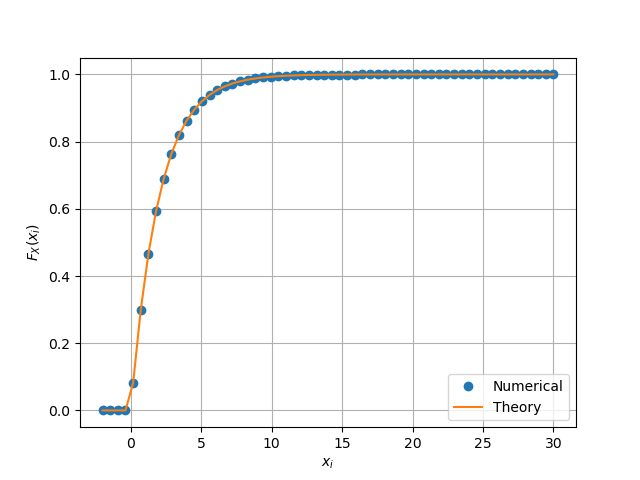
\includegraphics[scale=0.5]{/home/vijay/Digital_Communication/Figs/Chapter2/v_cdf_plot.png}  
\caption{The CDF of $V$}
\label{fig:log_uni_cdf}
\end{figure}

\item Find a theoretical expression for $F_V(x)$.\\
\solution We Know That,
\begin{flalign}
	F_V(x) &= P(V < x)&\\
	&= P(-2\ln\brak{1-U} < x)&\\
	&= P(U < 1 - e^{\frac{-x}{2}})&\\
	&= F_U(1 - e^{\frac{-x}{2}})
\end{flalign}

Using $F_U(x)$ from \eqref{eq:uniform_cdf}. We finally get
\begin{align}
	F_V(x) &=
	\begin{cases}
		0 & x < 0\\
		1 - e^{\frac{-x}{2}} & x \ge 0
	\end{cases}
\end{align} 

\end{enumerate}
\subsection{\textbf{Triangular Distribution}}
\begin{enumerate}[label=\thesubsection.\arabic*,ref=\thesubsection.\arabic{figure}]
%
\item Generate 
	\begin{align}
		T = U_1+U_2
	\end{align}
\solution T is generated using the following C programs.\\

\fbox{\parbox{85mm}{\href{https://github.com/SurabhiSeetha/Fwciith2022}{/Codes/Chapter2/coeffs.h}}}\\

\fbox{\parbox{85mm}{\href{https://github.com/SurabhiSeetha/Fwciith2022}{/Codes/Chapter2/tri$\_$gen.c}}}\\

\item Find the CDF of $T$.\\
\solution
The CDF of T is plotted in the Fig.\ref{fig:tri_cdf11} using the below Python Code\\ 

\fbox{\parbox{85mm}{\href{https://github.com/SurabhiSeetha/Fwciith2022}{/Codes/Chapter2/tri$\_$cdf$\_$plot.py}}}\\


\begin{figure}[!ht]
\centering
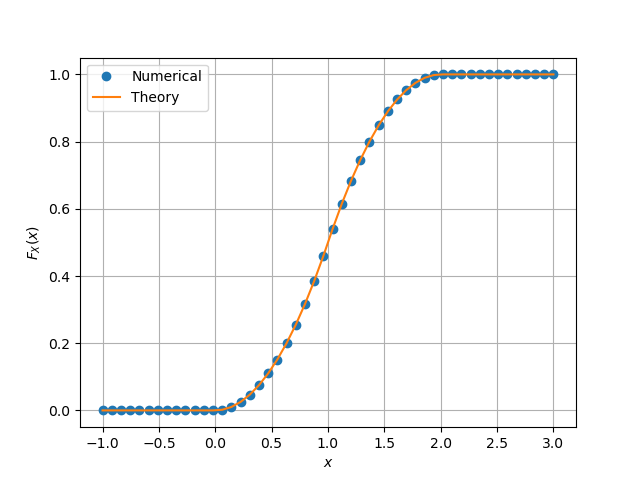
\includegraphics[scale=0.5]{/home/vijay/Digital_Communication/Figs/Chapter2/tri_cdf_plot.png} 
\caption{The CDF of $T$}
\label{fig:tri_cdf11}
\end{figure}


\item Find the PDF of $T$.\\
\solution: The PDF of T is plotted in the Fig.\ref{fig:tri_pdf11} using the below Python Code\\ 

\fbox{\parbox{85mm}{\href{https://github.com/SurabhiSeetha/Fwciith2022}{/Codes/Chapter2/tri$\_$pdf$\_$plot.py}}}\\


\begin{figure}[!ht]
\centering
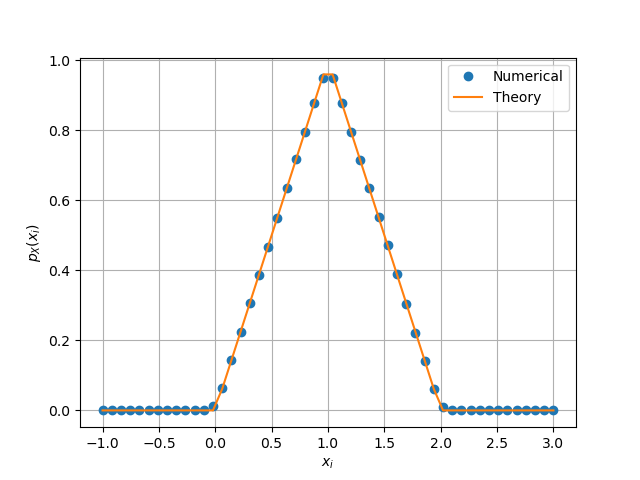
\includegraphics[scale=0.5]{/home/vijay/Digital_Communication/Figs/Chapter2/tri_pdf_plot.png} 
\caption{The PDF of $T$}
\label{fig:tri_pdf11}
\end{figure}

\item Find the theoretical expressions for the PDF and CDF of $T$.\\
\solution Since $T$ is the sum of the independant random variables $U1$ and $U2$, the PDF of $T$ is given by
\begin{flalign}
	p_T(x) &= p_{U1}(x) \ast p_{U2}(x)
\end{flalign}
Using the PDF of $U$ from \eqref{eq:uni_pdf}, we get the answer as
\begin{align}
	p_T(x) &=
	\begin{cases}
		0 & x < 0\\
		x & 0 \le x \le 1\\
		2-x & 1 \le x \le 2\\
		0 & x > 2
	\end{cases}
	\label{eq:tri_pdf}
\end{align}
The CDF of $T$ is calculated using \eqref{eq:pdf_to_cdf} where we put T instead of U and solve the integration. We finally arrive at the following result 
\begin{align}
	F_T(x) &=
	\begin{cases}
		0 & x < 0\\
		\frac{x^2}{2} & 0 \le x \le 1\\
		2x-\frac{x^2}{2}-1 & 1 \le x \le 2\\
		1 & x > 2
	\end{cases}
\end{align}

\item Verify your results through a plot. \\
\solution: The theoretical and simulated results of both CDF and PDF of the Triangular Distribution T have been compared and verified using the plots show in the Fig. \ref{fig:tri_cdf11}and \ref{fig:tri_pdf11} which were generated using Python.

\end{enumerate}

%%% chapter-3%%%
\section{Maximum Likelyhood Detection:BPSK}
\subsection{\textbf{Maximum Likelihood}}
\begin{enumerate}[label=\thesubsection.\arabic*,ref=\thesubsection.\arabic{figure}]
\item Generate equiprobable $X \in \cbrak{1,-1}$.\\

\solution The Random Variable X is generated using the following Python Code\\

\fbox{\parbox{85mm}{\href{https://github.com/SurabhiSeetha/Fwciith2022}{/Codes/Chapter3/eqprob.py}}}\\

\item Generate 
\begin{equation}
Y = AX+N,
\end{equation}
		where $A = 5$ dB,  and $N \sim \gauss{0}{1}$.\\


\solution The Random Variable Y is generated from the Random Variable X from the previous problem using the following Python Code\\

\fbox{\parbox{85mm}{\href{https://github.com/SurabhiSeetha/Fwciith2022}{/Codes/Chapter3/5$\_$1$\_$2.py}}}\\	
	
\item Plot $Y$ using a scatter plot.\\

\solution
The Python Code for the Scatter Plot of $Y$ is given below. The Corresponding plot is shown in the Fig.\ref{fig:scatter1} \\

\fbox{\parbox{85mm}{\href{https://github.com/SurabhiSeetha/Fwciith2022}{/Codes/Chapter3/5$\_$1$\_$3.py}}}\\

\
\begin{figure}[!ht]
\centering
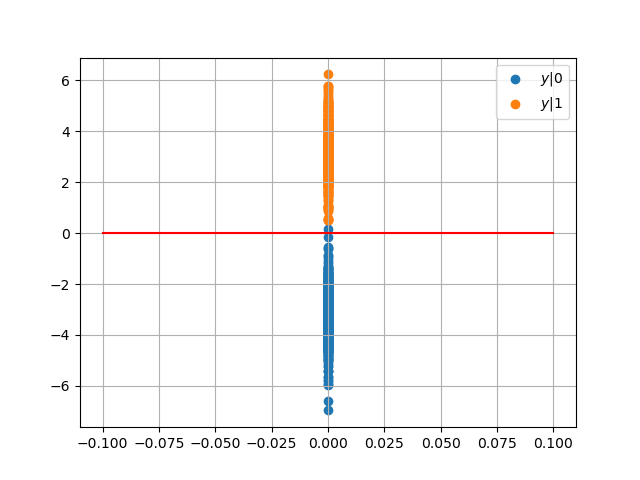
\includegraphics[scale=0.5]{/home/vijay/Digital_Communication/Figs/Chapter3/bpsk_scatter.png}  
\caption{The scatter plot of Y}
\label{fig:scatter1}
\end{figure}
\
	\item Guess how to estimate $X$ from $Y$.\\
	\solution 
	The Given Signal is represented by two signals\\
	'1' for X=1 and\\
	'0' for X=-1.
	according to decision rule $P(Y > y)$
	\begin{align}
        y \dec{1}{-1} 0 \label{eq:decision1}
        \end{align}
\item
\label{ml-ch4_sim}
Find 
\begin{equation}
	P_{e|0} = \pr{\hat{X} = -1|X=1}
\end{equation}
and 
\begin{equation}
	P_{e|1} = \pr{\hat{X} = 1|X=-1}	
\end{equation}\\
\solution From the previous solution \eqref{eq:decision1}, we can write
\begin{flalign*}
	\pr{\hat{X} = -1|X=1} &= \pr{Y < 0|X=1}&\\
	&= \pr{AX + N < 0|X=1}&\\ 
	&= \pr{A + N < 0}&\\
	&= \pr{N < -A}
\end{flalign*}
Similarly,
\begin{flalign*}
	\pr{\hat{X} = 1|X=-1} &= \pr{Y > 0|X=-1}&\\
	&= \pr{N > A}
\end{flalign*}
Since $N \sim \gauss{0}{1}$, i.e, it is Symmetric. We can write,
\begin{flalign}
	\label{eq:std_norm_symmetric}
	\pr{N < -A} &= \pr{N > A}&\\
	\label{eq:bpks_prob_err_cond}
	\implies P_{e|0} &= P_{e|1} 
\end{flalign}

 \item Find $P_e$ assuming that $X$ has equiprobable symbols.\\
 \solution \begin{align}
	P_e &= \pr{X=1}P_{e|1} + \pr{X=-1}P_{e|0}& \label{eq:Pe_of_X}
	\end{align}
	\text{assuming that $X$ is equiprobable,}\\
	\begin{align}
	P_e &= \frac{1}{2}P_{e|1} + \frac{1}{2}P_{e|0}
\end{align}
Substituting from \eqref{eq:bpks_prob_err_cond}
\begin{equation}
	P_e = \pr{N > A}
\end{equation}
Given a random varible $X \sim \gauss{0}{1}$ the Q-function is defined as
\begin{align}
	Q(x) &= \pr{X > x}\\
	\label{eq:q_func_integral}
	Q(x) &= \frac{1}{\sqrt{2\pi}} \int_x^\infty \exp\left(-\frac{u^2}{2}\right) \, du.
\end{align}
Using the above Q Function, $P_e$ can be rewritten as
\begin{equation}
	P_e = Q(A)
\end{equation} 
\item
Verify by plotting  the theoretical $P_e$ with respect to $A$ from 0 to 10 dB.\\
\solution 
The theoretical and simulated estimations of $P_e$ with respect to $A$ are plotted in the Fig \ref{fig:bpsk1}. Below is the python code for the plotting. \\

\fbox{\parbox{85mm}{\href{https://github.com/SurabhiSeetha/Fwciith2022}{/Codes/Chapter3/PevsA.py}}}\\	
	
\begin{figure}[!ht]
\centering
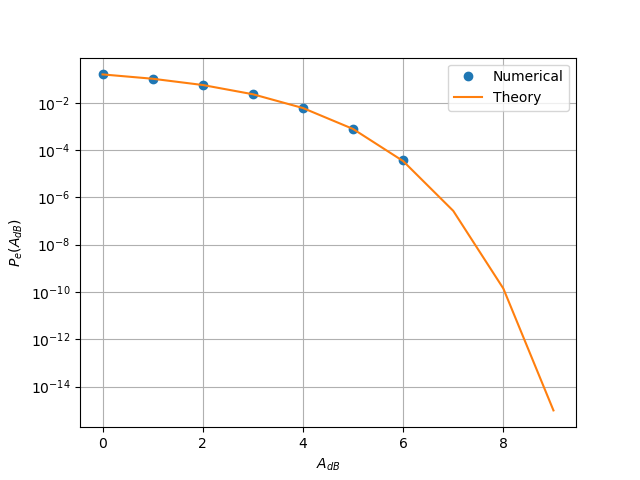
\includegraphics[scale=0.5]{/home/vijay/Digital_Communication/Figs/Chapter3/Pe_vs_A.png}   
\caption{$P_e$ of X wrt SNR(A)}
\label{fig:bpsk1}
\end{figure}

\item Now, consider a threshold $\delta$  while estimating $X$ from $Y$. Find the value of $\delta$ that maximizes the theoretical $P_e$.\\
\solution From \ref{eq:decision1} the decision rule, 
\begin{equation}
y \dec{1}{-1} \delta
\end{equation}
\begin{align*}
	P_{e|0} &= \pr{\hat{X} = -1|X=1}&\\
	&= \pr{Y < \delta|X=1}&\\
	&= \pr{AX + N < \delta|X=1}&\\ 
	&= \pr{A + N < \delta}&\\
	&= \pr{N < -A + \delta}&\\
	&= \pr{N > A - \delta}&\\
	&= Q(A-\delta)
\end{align*}
\begin{align*}
	P_{e|1} &= \pr{\hat{X} = 1|X=-1}&\\
	&= \pr{Y > \delta|X=-1}&\\
	&= \pr{N > A + \delta}&\\
	&= Q(A+\delta)
\end{align*}
From the Eq. \ref{eq:Pe_of_X} $P_e$ can be written as,
\begin{align}
	P_e &= \frac{1}{2}Q(A+\delta) + \frac{1}{2}Q(A-\delta)
\end{align}
Using the integral for Q-function from the equation \ref{eq:q_func_integral}, we get,
\begin{align}
	P_e &= k(\int_{A+\delta}^\infty \exp\left(-\frac{u^2}{2}\right) \, du + \int_{A-\delta}^\infty \exp\left(-\frac{u^2}{2}\right) \, du)
	\label{eq:Pe_in_q}
	\end{align}
	\text{where k is a constant}	\\
Differentiating \ref{eq:Pe_in_q}. wrt $\delta$ (using Leibniz's rule) and equating to $0$, we get
\begin{align}
	\exp\left(-\frac{(A+\delta)^2}{2}\right)-\exp\left(-\frac{(A-\delta)^2}{2}\right) &= 0&\\
	\frac{\exp\left(-\frac{(A+\delta)^2}{2}\right)}{\exp\left(-\frac{(A-\delta)^2}{2}\right)} &= 1&\\
	\exp\left(-\frac{(A+\delta)^2-(A-\delta)^2}{2}\right) &= 1&\\
	\exp\left(-2A\delta\right) &= 1&\\
	\intertext{Taking $\log$ on both sides}\\
	-2A\delta &= 0&\\
	\implies \delta &= 0
\end{align}
$\therefore P_e$ is maximum for $\delta = 0$
\item Repeat the above exercise when 

	\begin{align}
		p_{X}(0) = p
	\end{align}
	\solution Given $X$ is not equiprobable, hence $P_e$ is given by,
\begin{align}
	P_e &= (1-p)P_{e|1} + pP_{e|0}&\\
	&= (1-p)Q(A+\delta) + pQ(A-\delta)
\end{align}
Using the integral for Q-function from the equation \ref{eq:q_func_integral} we get,
\begin{align}
	P_e = k((1-p)\int_{A+\delta}^\infty \exp\left(-\frac{u^2}{2}\right) \, du + 
	p\int_{A-\delta}^\infty \exp\left(-\frac{u^2}{2}\right) \, du)
\end{align}
where $k$ is a constant.\\
differentiate $P_e$ wrt $\delta$ and equate to zero,
\begin{align}
	(1-p)\exp\left(-\frac{(A+\delta)^2}{2}\right)-p\exp\left(-\frac{(A-\delta)^2}{2}\right) &= 0&\\
	\exp\left(-\frac{(A+\delta)^2-(A-\delta)^2}{2}\right) &= \frac{p}{(1-p)}&\\
	\exp\left(-2A\delta\right) &= \frac{p}{(1-p)}&\\
	\intertext{Taking $\log$ on both sides we finally get,}
	\delta = \frac{1}{2A}\log\left(\frac{1}{p}-1\right)
	\label{eq:bpsk_decision_uneqi}
\end{align}

\item Repeat the above exercise using the MAP criterion.\\
\solution 
The MAP rule can be stated as
\begin{flalign}
\label{eq:map_rule}
\text{Set } \hat{x} &= x_i \text{ if} 
p_X(x_k)p_Y(y|x_k) \text{ is maximum for } k = i
\end{flalign}
But in the case of BPSK, the point of equality between $p_X(x=1)p_Y(y|x=1)$ and $p_X(x=-1)p_Y(y|x=-1)$ is the optimum threshold.\\
\
Assuming that this threshold is $\delta$, then we can formulate the below equations
\begin{flalign}
	pp_Y(y|x=1) > (1-p)p_Y(y|x=-1) &\text{ when } y > \delta \\
	pp_Y(y|x=1) < (1-p)p_Y(y|x=-1) &\text{ when } y < \delta 	
\end{flalign}
The Python code for visualizing the above set of inequalities is given below.\\

\fbox{\parbox{85mm}{\href{https://github.com/SurabhiSeetha/Fwciith2022}{/Codes/Chapter3/bpsk.py}}}\\	

The plot of the above inequalities for $p = 0.3$ and $A = 3$ is show in the Fig \figref{fig:bpsk_map_density} 
\begin{figure}[!ht]
\centering
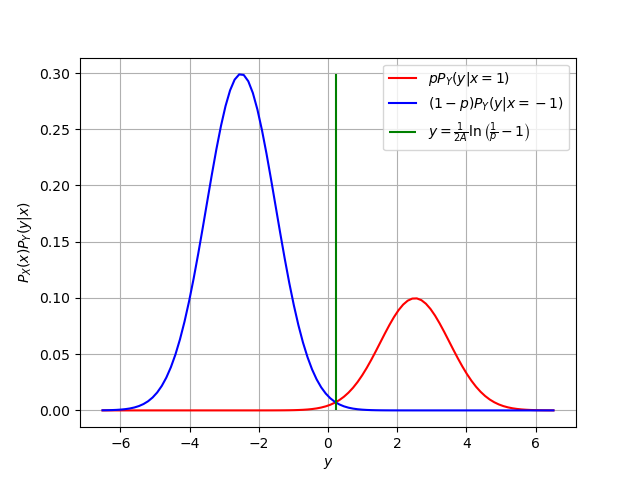
\includegraphics[width=\columnwidth]{/home/vijay/Digital_Communication/Figs/Chapter3/bpsk_map.png}
\caption{$p_X(X=x_i)p_Y(y|x=x_i)$ versus $y$ plot for $X \in \{-1,1\}$}
\label{fig:bpsk_map_density}
\end{figure}

Given $Y=AX+N$ where $N \sim \gauss{0}{1}$, the optimum threshold is found to be,

\begin{equation}
	y_{eq} = \delta = \frac{1}{2A}\ln\left(\frac{1}{p}-1\right)
\end{equation}
which is same as $\delta$ obtained in problem \ref{eq:bpsk_decision_uneqi}

\end{enumerate}

%%%chapter-4%%
\section{Transformation of random variables}	
\subsection{\textbf{Gaussian to Other}}
\begin{enumerate}[label=\thesubsection.\arabic*,ref=\thesubsection.\arabic{figure}]
\item
Let $X_1 \sim  \gauss{0}{1}$ and $X_2 \sim  \gauss{0}{1}$. Plot the CDF and PDF of
%
\begin{equation}
V = X_1^2 + X_2^2
\end{equation}
\solution 
The CDF and PDF of V are plotted using the following codes respectively. The corresponding plots are show in the Figures \ref{fig:gauss_cdf1} , \ref{fig:gauss_pdf1} respectively.\\

\fbox{\parbox{85mm}{\href{https://github.com/SurabhiSeetha/Fwciith2022}{/Codes/Chapter4/sq$\_$sum$\_$cdf.py}}}\\	

\fbox{\parbox{85mm}{\href{https://github.com/SurabhiSeetha/Fwciith2022}{/Codes/Chapter4/sq$\_$sum$\_$pdf.py}}}\\	

\begin{figure}[!ht]
\centering
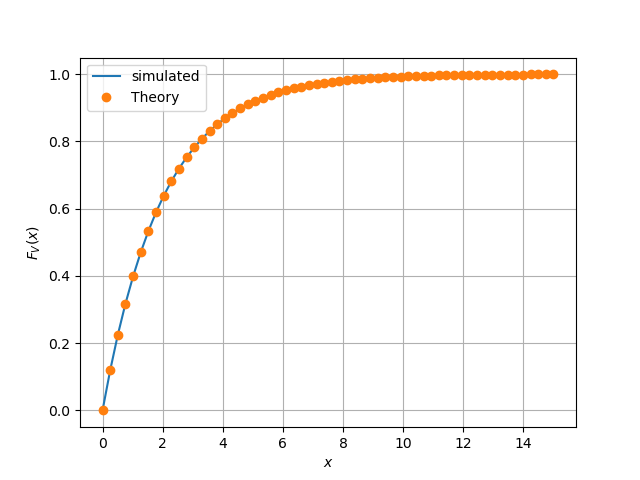
\includegraphics[scale=0.5]{/home/vijay/Digital_Communication/Figs/Chapter4/chisq_cdf.png}  
\caption{The CDF of $V$}
\label{fig:gauss_cdf1}
\end{figure}
\begin{figure}[!ht]
\centering
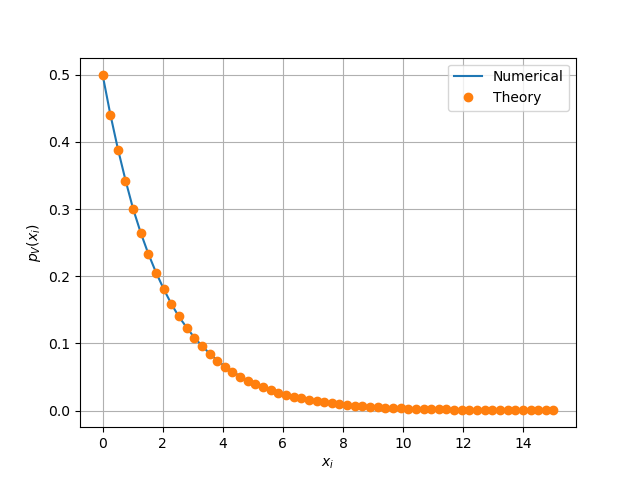
\includegraphics[scale=0.5]{/home/vijay/Digital_Communication/Figs/Chapter4/chisq_pdf.png}   
\caption{The PDF of $V$}
\label{fig:gauss_pdf1}
\end{figure}

\item
If
%
\begin{equation}
F_{V}(x) = 
\begin{cases}
1 - e^{-\alpha x} & x \geq 0 \\
0 & x < 0,
\end{cases}
\label{eq:chisq2_cdf_gen}
\end{equation}
%
find $\alpha$.\\
\solution Let $Z=X^2$ where $X \sim \gauss{0}{1}$. The CDF of $Z$ can eb defined as,
\begin{flalign*}
	P_Z(z) &= \pr{Z < z}&\\
	&= \pr{X^2 < z}&\\
	&= \pr{-\sqrt{z} < X < \sqrt{z}}&\\
	&= \int_{-\sqrt{z}}^{\sqrt{z}} p_X(x)  \,dx 
\end{flalign*}
From the Eq. \eqref{eq:cdf_to_pdf}, the PDF of $Z$ is given by
\begin{align}
	\nonumber
	\frac{d}{dz}P_Z(z) &= p_Z(z)\\
	\label{eq:square_pdf_gen}
	= \frac{p_X(\sqrt{z})+p_X(-\sqrt{z})}{2\sqrt{z}} & \text{ [ By Lebniz's rule ]} 
\end{align}
By Substituting the gaussian function $p_X(x) = \frac{1}{\sqrt{2\pi}}e^{-\frac{x^2}{2}}$ in \eqref{eq:square_pdf_gen} we get,
\begin{equation}
	p_Z(z) =
	\begin{cases}
	\frac{1}{\sqrt{2\pi z}}e^{-\frac{z}{2}} & z \ge 0\\
	0 & z < 0
	\end{cases} 
	\label{eq:chisq_pdf}
\end{equation}
The PDF of $X_1^2$ and $X_2^2$ are given by \eqref{eq:chisq_pdf}. Since $V$ is the sum of two independant random variables we can write,
\begin{flalign*}
	p_V(v) &= p_{X_1^2}(x_1) \ast p_{X_2^2}(x_2)&\\
	&= \frac{1}{2\pi} \int_{0}^{v} \frac{e^{-\frac{x}{2}}}{\sqrt{x}}\frac{e^{-\frac{v-x}{2}}}{\sqrt{v-x}}  \,dx&\\
	&= \frac{e^{-\frac{v}{2}}}{2\pi} \int_{0}^{v} \frac{1}{\sqrt{x(v-x)}}  \,dx&\\
	&= \frac{e^{-\frac{v}{2}}}{2\pi} \sbrak{-\arcsin\left(\dfrac{v-2x}{v}\right)}_0^v&\\
	&= \frac{e^{-\frac{v}{2}}}{2\pi} \pi&\\
	&= \frac{e^{-\frac{v}{2}}}{2} \text{ for } v \ge 0
\end{flalign*}
$F_V(v)$ can be obtained from $p_V(v)$ using the equation \eqref{eq:pdf_to_cdf}
\begin{flalign}
	\nonumber
	F_V(v) &= \frac{1}{2} \int_{0}^{v} \exp\left(-\frac{v}{2}\right)&\\
	\label{eq:chisq2_cdf}
	&= 1-\exp\left(-\frac{v}{2}\right) \text{ for } v \ge 0
\end{flalign}
Comparing \eqref{eq:chisq2_cdf} with \eqref{eq:chisq2_cdf_gen}, $\alpha = \frac{1}{2}$ 
%
\item
\label{ch3_raleigh_sim}
Plot the CDF and PDf of
%
\begin{equation}
A = \sqrt{V}
\end{equation}\\
\solution
The CDF and PDF of A are plotted using the following codes respectively. The corresponding plots are show in the Figures \ref{fig:gauss_othr_cdf2},\ref{fig:gauss_othr_pdf2} respectively.\\

\fbox{\parbox{85mm}{\href{https://github.com/SurabhiSeetha/Fwciith2022}{/Codes/Chapter4/sqroot$\_$cdf.py}}}\\	

\fbox{\parbox{85mm}{\href{https://github.com/SurabhiSeetha/Fwciith2022}{/Codes/Chapter4/sqroot$\_$pdf.py}}}\\	

\begin{figure}[!ht]
\centering
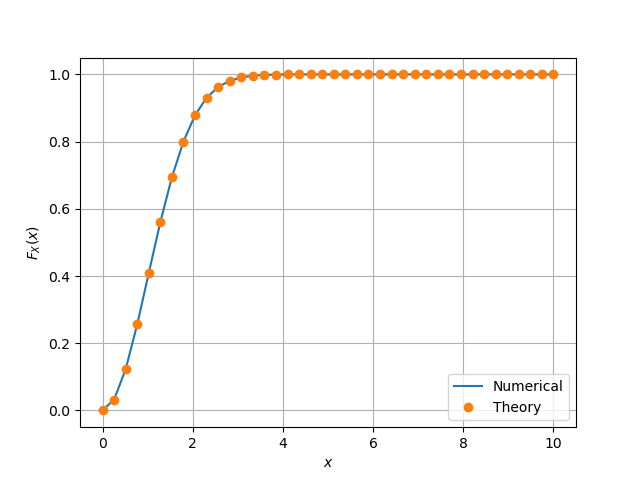
\includegraphics[scale=0.5]{/home/vijay/Digital_Communication/Figs/Chapter4/rayleigh_cdf.png}     
\caption{The CDF of $A$ }
\label{fig:gauss_othr_cdf2}
\end{figure}
\begin{figure}[!ht]
\centering
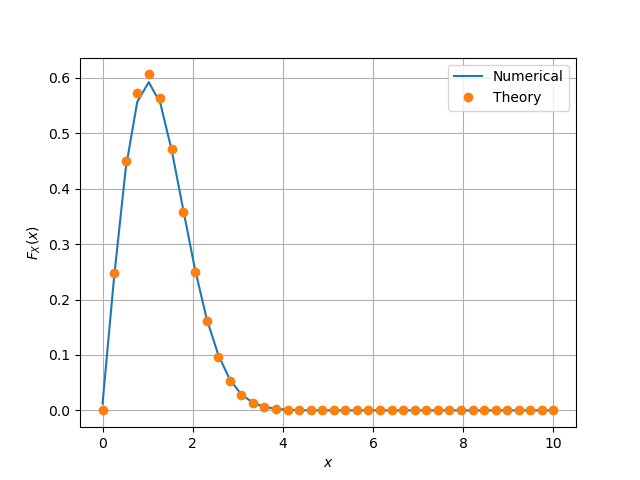
\includegraphics[scale=0.5]{/home/vijay/Digital_Communication/Figs/Chapter4/rayleigh_pdf.png}     
\caption{The PDF of $A$ }
\label{fig:gauss_othr_pdf2}
\end{figure}
\end{enumerate}


\subsection{\textbf{Conditional Probability}}
\begin{enumerate}[label=\thesubsection.\arabic*,ref=\thesubsection.\arabic{figure}]
\item
Plot 
\begin{equation}
\label{eq:ch4_1}
P_e = \pr{\hat{X} = -1|X=1}
\end{equation}
%
for 
\begin{equation}
Y = AX+N,
\end{equation}
where $A$ is Raleigh with $E\sbrak{A^2} = \gamma, N \sim \gauss{0}{1}, X \in \brak{-1,1}$ for $0 \le \gamma \le 10$ dB.
\item
Assuming that $N$ is a constant, find an expression for $P_e$.  Call this $P_e(N)$\\
\solution Assuming the decision rule in \eqref{eq:decision1}, when $N$ is constant, $P_e$ can be calculated by the following steps, 
\begin{align}
\hat{X} = 
\begin{cases}
+1 & Y>0\\
-1 & Y<0
\end{cases}
\end{align}
For $X = 1$, 
\begin{align}
Y &= A + N\\
P_e &= \pr{\hat{X} = -1|X=1} \\
&= \pr{Y<0 |X=1}\\
&= \pr{AX + N < 0|X=1}&\\ 
	\label{eq:prob_err_rayleigh_gen}
	&= \pr{A + N < 0}&\\
	&= \pr{N < -A}\\
	\label{eq:prob_err_bpsk_rayleigh_cdf}
	&=
	\begin{cases}
	F_A(-N) & N \ge 0\\
	0 & N < 0
	\end{cases}
\end{align}
By definition For a Rayleigh random variable $X$ with $E\sbrak{X^2} = \gamma$, the PDF and CDF are given by,
\begin{align}
\label{eq:rayleigh_pdf}
f_A(x) = 
\frac{x}{\gamma}\exp\brak{{-\frac{x^2}{\gamma}}} \text{ for } x \ge 0\\
\label{eq:rayleigh_cdf}
F_A(X) = 1-\exp\left(-\frac{x^2}{\gamma}\right) \text{ for } x \ge 0
\end{align}
If $N<0, f_A(x) = 0$. Then,
\begin{align}
 P_e=0  
\end{align}
If $N \geq 0$. Then,
\begin{align}
 P_e(N) &=\int_{-\infty}^{-N} f_A(x)dx\\
 &=\int_{-\infty}^{0} 0dx+\int_{0}^{-N} f_A(x)dx\\
 &=\int_{0}^{-N} \frac{x}{\gamma}\exp\brak{{-\frac{x^2}{\gamma}}}dx\\
 &=1-\exp{\brak{-\frac{N^2}{\gamma}}}
\end{align}
Therefore,
\begin{align}\label{pe(N)}
P_e(N) = 
\begin{cases}
1-\exp\brak{{-\frac{N^2}{\gamma}}} & N \geq0\\
0 & otherwise
\end{cases}
\end{align}
%
\item
For a function $g$,
\begin{equation}
\label{prob:ch4_g}
E\sbrak{g(X)} = \int_{-\infty}^{\infty}g(x)p_{X}(x)\, dx
\end{equation}
%
Find $P_e = E\sbrak{P_e(N)}$.
\\
\solution
Since $N \sim \gauss{0}{1}$ ,
\begin{align}
  p_N(x)= \frac{1}{\sqrt{2\pi}}\exp \brak{-\frac{x^2}{2} }
\end{align}
And from \eqref{pe(N)} 
\begin{align}
    P_e(x)=
    \begin{cases}
1-\exp\brak{{-\frac{x^2}{\gamma}}} & x\geq0\\
0 & otherwise
\end{cases}
\end{align}

\begin{align}
 P_e=E\sbrak{P_e(N)} = \int_{-\infty}^{\infty}P_e(x)p_{N}(x)\, dx  
\end{align}
We know that for any even function, we can write
\begin{align}
\int_{-\infty}^{\infty}f(x)=2\int_{-\infty}^{0}f(x)   
\end{align}
we get
\begin{align}
  P_e= \frac{1}{\sqrt{2\pi}}\int_{-\infty}^{0}\exp \brak{ -\frac{x^2}{2}} \brak{1-\exp \brak{ -\frac{x^2}{\gamma}} } dx
\end{align}
\begin{multline}
	P_e = \frac{1}{\sqrt{2\pi}}\int_{0}^{\infty} e^{-\frac{x^2}{2}}  \,dx \\ - \frac{1}{\sqrt{2\pi}}\int_{0}^{\infty} \exp\left(-x^2\left(\frac{1}{\gamma}+\frac{1}{2}\right)\right)  \,dx
\end{multline}
\begin{align}
\therefore P_e = \frac{1}{2} - \frac{1}{2}\sqrt{\frac{\gamma}{2+\gamma}}
\end{align}


\item
Plot $P_e$ in problems \ref{eq:ch4_1} and \ref{prob:ch4_g} on the same graph w.r.t $\gamma$.  Comment. \\
\solution $P_e$ w.r.t $\gamma$ plot is show in the \figref{fig:Pe_gamma1}. The value of $P_e$ is much higher when the channel %
gain $A$ is Rayleigh distributed than the case where $A$ is a constant (compare with \figref{fig:bpsk1}).\\


\fbox{\parbox{85mm}{\href{https://github.com/SurabhiSeetha/Fwciith2022}{/Codes/Chapter4/pe$\_$vs$\_$gamma.py}}}\\	

\begin{figure}[!ht]
\centering
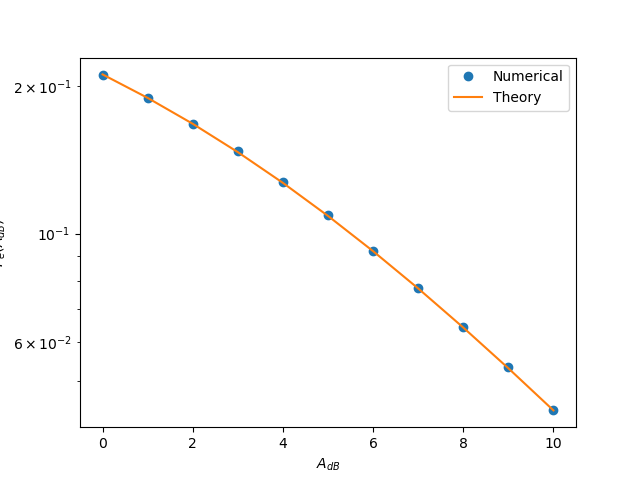
\includegraphics[scale=0.5]{/home/vijay/Digital_Communication/Figs/Chapter4//Pe_vs_gamma.png}      
\caption{The $P_e$ wrt $\gamma$ }
\label{fig:Pe_gamma1}
\end{figure}

\end{enumerate}

\section{Bivariate Random Variables:FSK}
\subsection{\textbf{Two Dimensions}}
Let 
\begin{equation*}
\mbf{y} = A\mbf{x} + \mbf{n},
\end{equation*}
where 
\begin{align*}
x &\in \brak{\mbf{s}_0,\mbf{s}_1}, 
\mbf{s}_0 = 
\begin{pmatrix}
1 
\\
0
\end{pmatrix},
\mbf{s}_1 = 
\begin{pmatrix}
0 
\\
1
\end{pmatrix}
\\
\mbf{n} &= 
\begin{pmatrix}
n_1
\\
n_2
\end{pmatrix},
n_1,n_2 \sim \gauss{0}{1}.
\end{align*}
\begin{enumerate}[label=\thesubsection.\arabic*,ref=\thesubsection.\arabic{figure}]
%%
\item
\label{ch5_fsk}
Plot 
%
\begin{equation}
\mbf{y}|\mbf{s}_0 \text{ and } \mbf{y}|\mbf{s}_1
\end{equation}
%
on the same graph using a scatter plot.\\
\solution The scatter plot for $\mbf{x} = \mbf{s}_0$ and $\mbf{x} = \mbf{s}_1$ shown in Fig. \ref{fig:scatter_2} is generated by the following Python code.\\

\fbox{\parbox{85mm}{\href{https://github.com/SurabhiSeetha/Fwciith2022}{/Codes/Chapter5/bfsk$\_$scatter.py}}}\\	

\begin{figure}[!ht]
\centering
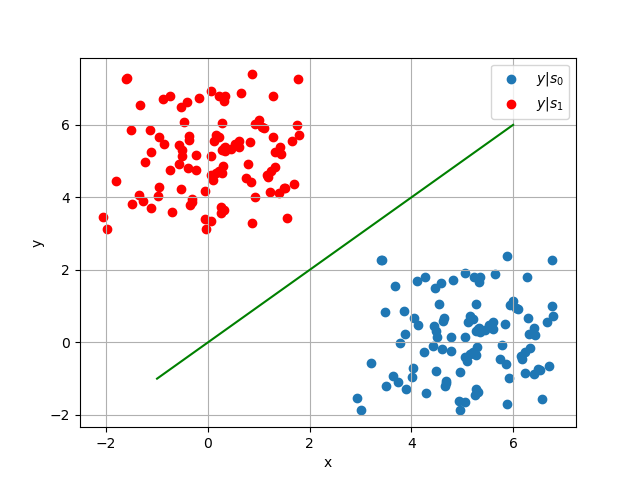
\includegraphics[scale=0.5]{/home/vijay/Digital_Communication/Figs/Chapter5/bfsk_scatter.png}     
\caption{Y scatter plot }
\label{fig:scatter_2}
\end{figure}
\item
For the above problem, find a decision rule for detecting the symbols $\mbf{s}_0 $ and $\mbf{s}_1$.\\
\solution 

    For a bivariate gaussian distribution,
    {\small
    \begin{multline}
    \label{eq:bivariate}
    p(x,y)= \frac{1}{2\pi \sigma_x\sigma_y\sqrt{1-\rho^2}}\exp\lsbrak{-\frac{1}{2\brak{1-\rho^2}}}
    \\
    \times \rsbrak{\cbrak{\frac{\brak{x-\mu_x}^2}{\sigma_x^2}+\frac{\brak{y-\mu_y}^2}{\sigma_y^2}-\frac{2\rho\brak{x-\mu_x}\brak{y-\mu_y}}{\sigma_x\sigma_y}}}
    \end{multline}
    }
    %
    where
    %
    \begin{align}
\mbf{\mu}=\begin{pmatrix}
\mbf{\mu_x} \\
\mbf{\mu_y}
\end{pmatrix} , \mbf{\Sigma} = \begin{pmatrix}
\sigma_x^2 & \rho\sigma_x\sigma_y \\
    \rho\sigma_x\sigma_y & \sigma_y^2
\end{pmatrix} \\
\rho = \frac{E\sbrak{\brak{x - \mu_x}\brak{y-\mu_y}}}{\sigma_x\sigma_y}.
    %  
    \end{align}
        \begin{align}
        \mbf{y}|s_0 &= 
        \begin{pmatrix}
        A+n_1 \\
        n_2
        \end{pmatrix}\\
        \mbf{y}|s_1 &=  
        \begin{pmatrix}
        n_1 \\
        A+n_2
        \end{pmatrix}
        \end{align}

$\vec{y}|\vec{s}_i$ is a random vector with each of its components normally distributed. The PDF of $\vec{y}|\vec{s}_i$ is given by,
\begin{equation}
	p_{\vec{y}|\vec{s}_i}\brak{\vec{y}} = \frac{1}{2\pi\sqrt{\mydet{\vec{\Sigma}}}} \exp\brak{-\frac{1}{2}\brak{\vec{y}-\vec{s}_i}^\top \vec{\Sigma}^{-1} \brak{\vec{y}-\vec{s}_i}}
\end{equation}
Where $\vec{\Sigma}$ is the covariance matrix. Substituting $\vec{\Sigma} = \sigma \vec{I}$,
\begin{align}
	p_{\vec{y}|\vec{s}_i}\brak{\vec{y}} &= \frac{1}{2 \pi \sigma} \exp\brak{-\frac{1}{2 \sigma}\brak{\vec{y}-\vec{s}_i}^\top \vec{I} \brak{\vec{y}-\vec{s}_i}}\\
	&= \frac{1}{2 \pi \sigma} \exp\brak{-\frac{1}{2 \sigma}\brak{\vec{y}-\vec{s}_i}^\top \brak{\vec{y}-\vec{s}_i}}
\end{align}
  
         For equiprobably symbols, the MAP criterion is defined as
        %
        \begin{align}
        \label{eq:map_bfsk_dec}
        p\brak{\vec{y}|s_0} &\dec{s_0}{s_1} p\brak{\vec{y}|s_1}
        \end{align}  
         Since there are only two possible symbols %
$\vec{s}_0$ and $\vec{s}_1$, the optimal decision criterion is found by equating $p_{\vec{y}|\vec{s}_0}$ and $p_{\vec{y}|\vec{s}_1}$.
\begin{align}
	p_{\vec{y}|\vec{s}_0} &= p_{\vec{y}|\vec{s}_1}
\end{align}
\begin{multline}
	\implies \exp\brak{-\frac{1}{2 \sigma}\brak{\vec{y}-\vec{s}_0}^\top \brak{\vec{y}-\vec{s}_0}} = \\
	\exp\brak{-\frac{1}{2 \sigma}\brak{\vec{y}-\vec{s}_1}^\top \brak{\vec{y}-\vec{s}_1}}
\end{multline}
	
\begin{align}
	\implies \brak{\vec{y}-\vec{s}_0}^\top \brak{\vec{y}-\vec{s}_0} &= \brak{\vec{y}-\vec{s}_1}^\top \brak{\vec{y}-\vec{s}_1}\\
	\implies \vec{y}^\top\vec{y} - 2\vec{s}_0^\top \vec{y} + \vec{s}_0^T\vec{s}_0 &= \vec{y}^\top\vec{y} - 2\vec{s}_1^\top \vec{y} + \vec{s}_1^T\vec{s}_1\\
	\implies 2\brak{\vec{s}_1-\vec{s}_0}^\top \vec{y} &= \norm{\vec{s}_1}^2 - \norm{\vec{s}_0}^2\\
	\implies \brak{\vec{s}_1-\vec{s}_0}^\top \vec{y} &= 0\\
	\implies \myvec{-1\\1}^\top \vec{y} &= 0
\end{align}
        On simplifying, we get the decision rule is
        \begin{align}
        \label{eq:decision_rule}
        y_1 \dec{s_0}{s_1} y_2
        \end{align}
\item
Plot 
\begin{equation} 
P_e = \pr{\hat{\mbf{x}} = \mbf{s}_1|\mbf{x} = \mbf{s}_0}
\end{equation}
with respect to the SNR from 0 to 10 dB.\\
\solution 
The Fig. \ref{fig:Pe_snr2} Shows the $P_e$ vs SNR plot for Theoretical and Numerically Estimated values generated using the Python code give below\\

\fbox{\parbox{85mm}{\href{https://github.com/SurabhiSeetha/Fwciith2022}{/Codes/Chapter5/pe$\_$vs$\_$snr.py}}}\\	

\begin{figure}[!ht]
\centering
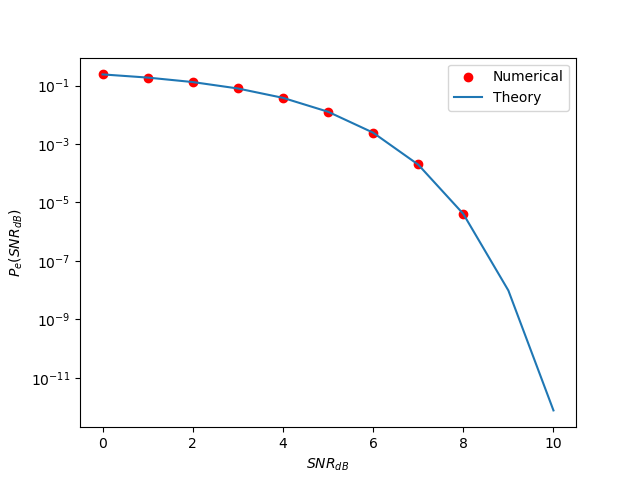
\includegraphics[scale=0.5]{/home/vijay/Digital_Communication/Figs/Chapter5/pe_vs_snr.png}     
\caption{Pe vs SNR }
\label{fig:Pe_snr2}
\end{figure}

\item
Obtain an expression for $P_e$. Verify this by comparing the theory and simulation plots on the same graph.\\
\solution Using the decision rule from \eqref{eq:decision_rule},    
	\begin{align}
P_e &= \pr{\hat{\mbf{x}} = \mbf{s}_1|\mbf{x} = \mbf{s}_0}\\\nonumber
	&= \pr{y_1 < y_2|\mbf{x} = \mbf{s}_0}\\\nonumber
	&= \pr{A+n_1 < n_2}\\
	\label{eq:prob_error_fsk_inter}
	&= \pr{n_1-n_2 < -A}\\
    &= \pr{n_2 - n_1 > A}
    \end{align}
    Let $Z = n_1-n_2$ where $n_1, n_2 \sim \gauss{0}{\sigma^2}$. The PDF of X is given by,
\begin{align}	
	p_Z(z) &= p_{n_1}(n_1) \ast p_{-n_2}(n_2)\\
	&= \frac{1}{2\pi\sigma^2}\int_{-\infty}^{\infty} e^{-\frac{t^2}{2\sigma^2}}e^{-\frac{(t-z)^2}{2\sigma^2}}  \,dt\\
	\label{eq:std_gauss_diff_pdf_fsk}
	&= \frac{e^{-\frac{z^2}{2(\sqrt{2}\sigma)^2}}}{\sqrt{2\pi}\sqrt{2}\sigma}
\end{align}    
Hence we have, $Z \sim \gauss{0}{2\sigma^2}$.\\
    \
From \eqref{eq:prob_error_fsk_inter} we can write,
    \begin{align}
     P_e &= \pr{Z > A}&\\
   &= \pr{\sqrt{2}w > A} \\
    &=  \pr{w > \dfrac{A}{\sqrt{2}}}
    \end{align}
    \
Where w $\sim \gauss{0}{1}$,\\
\
    Now, Substituting $\sigma=1$, $Z \sim \gauss{0}{2}$ in \eqref{eq:std_gauss_diff_pdf_fsk} we get,
    \begin{align}
	&= \frac{1}{\sqrt{2\pi}}\int_{\frac{A}{\sqrt{2}}}^{\infty} \exp\left(-\frac{x^2}{2}\right)  \,dx \\   
    \Rightarrow P_e &= \qfunc{\frac{A}{\sqrt{2}}}
    \end{align}
    
    The comparison of theoretical and simulated values can be observed in the $P_e$ vs SNR Graph shown in the Fig.\ref{fig:Pe_snr2}.
          
\end{enumerate}


\end{document}